\section{General Disagreement}

In this section we provide some details on general disagreement as discussed in Section IV.A in the paper. Specifically, as in the paper let $\Delta^i_{s,t}$ be the estimation error  at time $t$ of an agent of type $i$ born at time $s$. As before, the agents' perceived shocks are related to the true shock in the following way:
\begin{equation}
	dz^i_{s,t} = dz_{\alpha,t} - \Delta^i_{s,t}dt.
\end{equation}
The likelihood ratio, $\eta^i_{s,t}$, which represents the change of measure between the belief of agent $i$ born at time $s$ at time $t$ and the data generating probability measure has the dynamics
\begin{equation}
	d\eta^i_{s,t} = \Delta^i_{s,t} \eta^i_{s,t}dz_{\alpha,t}.
\end{equation}
We now provide details of Proposition 10 in the paper. First, from the FOC we have that:
\begin{equation}\label{IAoptimalconsumption}
	 c^i_{s,t} =c^i_{s,s} e^{-\rho_i \left(t-s\right)}\frac{\eta^i_{s,t}}{\eta^i_{s,s}} \frac{\xi_{s}}{\xi_{t}}
\end{equation}
Inserting optimal consumption given in Equation (\ref{IAoptimalconsumption}) into the market clearing condition we get
\begin{eqnarray}
	Y_t &=& \int_{-\infty}^{t} \nu e^{-\nu\left(t-s\right)}\left(\alpha_s c^a_{s,s} e^{-\rho_a \left(t-s\right)}\frac{\eta^a_{s,t}}{\eta^a_{s,s}} \frac{\xi_{s}}{\xi_{t}} + \left(1-\alpha_s\right)c^b_{s,s} e^{-\rho_b \left(t-s\right)}\frac{\eta^b_{s,t}}{\eta^b_{s,s}} \frac{\xi_{s}}{\xi_{t}}\right)ds \nonumber \\
	\xi_t Y_t &=& \int_{-\infty}^{t} \nu e^{-\nu\left(t-s\right)}\left(\alpha_s \beta^a_{s}e^{-\rho_a \left(t-s\right)}\frac{\eta^a_{s,t}}{\eta^a_{s,s}} + \left(1-\alpha_s\right)\beta^b_s e^{-\rho_b \left(t-s\right)}\frac{\eta^b_{s,t}}{\eta^b_{s,s}}\right)\xi_s Y_s ds \nonumber \\
		X_t &=& \int_{-\infty}^{t} \nu e^{-\nu\left(t-s\right)}\left(\alpha_s \beta^a_{s}e^{-\rho_a \left(t-s\right)}\frac{\eta^a_{s,t}}{\eta^a_{s,s}} + \left(1-\alpha_s\right)\beta^b_s e^{-\rho_b \left(t-s\right)}\frac{\eta^b_{s,t}}{\eta^b_{s,s}}\right)X_s ds, 
\end{eqnarray}
where $X_t = \xi_t Y_t$ implying $\xi_t = \frac{X_t}{Y_t}$. As before, we get for the consumption share of all patient investors:  $f_t = \int_{-\infty}^{t} \nu e^{-\nu\left(t-s\right)}\left(\alpha_s \beta^a_{s}e^{-\rho_a \left(t-s\right)}\frac{\eta^a_{s,t}}{\eta^a_{s,s}}\right)\frac{X_s}{X_t} ds$. An application of Ito's lemma 
gives
\begin{eqnarray}
	dX_t &=& X_t\left( \nu\left(\alpha_t \beta^a_t + \left(1-\alpha_t\right)\beta^b_t - 1\right)  - \rho_a f_t - \rho_b \left(1-f_t\right)\right) dt  \nonumber \\
	&&+ X_t\left(\bar{\Delta}^{a}_t f_t + \bar{\Delta}^b_t \left(1-f_t\right)\right)dZ_{\alpha,t},
\end{eqnarray}
where 
\begin{equation}
	\bar{\Delta}^i_t = \int_{-\infty}^{t} \bar{f}^i_{s,t} \Delta^i_{s,t}ds,  \qquad i=a,b,
\end{equation}
where  the within group consumption share densities are
\begin{eqnarray}
	\bar{f}^a_{s,t} &=&\left(\frac{1}{f_t}\right)\nu e^{-\left(\rho^a+\nu\right)\left(t-s\right)} \alpha_s \beta^a_{s}\left(\frac{\eta^a_{s,t}}{\eta^a_{s,s}}\right)\left(\frac{Y_s}{Y_t}\right)\left(\frac{\xi_s}{\xi_t}\right)\\
	\bar{f}^b_{s,t} &=& \left(\frac{1}{1-f_t}\right)\nu e^{-\left(\rho^b+\nu\right)\left(t-s\right)} \left(1-\alpha_s\right) \beta^b_{s}\left(\frac{\eta^b_{s,t}}{\eta^b_{s,s}}\right)\left(\frac{Y_s}{Y_t}\right)\left(\frac{\xi_s}{\xi_t}\right).
\end{eqnarray}
An application of Ito's lemma to $\xi_t = \frac{X_t}{Y_t}$ yields the following. 

\begin{prop}\label{SDFgeneralDIS}
The real short rate, $r_t$, and the market price of supply shocks, $\theta_{Y,t}$, take the same form as before and are given Proposition \ref{prop_rtandtheta}. The market price of demand shocks is 
\begin{equation}
\theta_{\alpha,t} %= - \bar{\Delta}_t  
= -\left(f_t \bar{\Delta}^a_t + \left(1-f_t\right)\bar{\Delta}^b_t\right), 
\end{equation}
where $f_t$ is the fraction of output consumed by all agents of type $a$. The within type $i$ consumption share weighted average estimation error is 
\begin{equation}
	\bar{\Delta}^i_t = \int_{-\infty}^{t} \bar{f}^i_{s,t} \Delta^i_{s,t}ds,  \qquad i=a,b,
\end{equation}
where  the within group consumption share densities are
\begin{eqnarray}
	\bar{f}^a_{s,t} &=&\left(\frac{1}{f_t}\right)\nu e^{-\left(\rho^a+\nu\right)\left(t-s\right)} \alpha_s \beta^a_{s}\left(\frac{\eta^a_{s,t}}{\eta^a_{s,s}}\right)\left(\frac{Y_s}{Y_t}\right)\left(\frac{\xi_s}{\xi_t}\right)\\
	\bar{f}^b_{s,t} &=& \left(\frac{1}{1-f_t}\right)\nu e^{-\left(\rho^b+\nu\right)\left(t-s\right)} \left(1-\alpha_s\right) \beta^b_{s}\left(\frac{\eta^b_{s,t}}{\eta^b_{s,s}}\right)\left(\frac{Y_s}{Y_t}\right)\left(\frac{\xi_s}{\xi_t}\right)
\end{eqnarray}
with $\beta^i_t = \left(\rho^i + \nu\right)\phi_t$ and the wealth-consumption ratio, $\phi_t$, as before. The stock price- and console dynamics are the same as in the baseline model where the constant disagreement, $\Delta$, is replaced with the stochastic disagreement $\Delta_t= \bar{\Delta}^a_t - \bar{\Delta}^b_t$. 
\end{prop}

The consumption share, $f_t$, is still an endogenous state variable but the within group consumption share weighted estimation errors replace the constant estimation errors from the previous section. Importantly, the risk-free rate and market prices of risk take similar forms as in the case without learning. Although it is sufficient to know $\alpha_t$, $f_t$ and $\bar{\Delta}_t$ to characterize the equilibrium at any point in time, the dynamics of $f_t$ and $\bar{\Delta}_t$ do not form a Markov system, but require the knowledge of every agent's belief. We now consider a special case where agents learn from their own experience. 

\subsection{Demand Disagreement with Learning from Experience}

In the baseline, model we made two assumptions about preferences and beliefs. First, there is a strong link between preferences and beliefs as agents disagree across but not within preference types. Second, agents do not learn. In this section, we relax both of these assumptions by allowing agents to learn from their own experience as in \cite{EGH18}. 

We assume that an agent of type $i$ born at time $s$ has a normally distributed prior about the long-run mean of $l_t$, with mean $\bar{l}^i$ and variance $V$. Hence, everyone has the same prior variance, $V$, but patient and impatient agents might have different prior means, $\bar{l}^i$. The next proposition characterizes the time-t estimation error of an agent born at time $s$.
\begin{prop}\label{LearningEstimationError}
The time-$t$ estimation error of an agent of type $i=a,b$ born at time $s$ is 
\begin{equation}
	 \Delta^i_{s,t} = \frac{\sigma_{A}^2}{\sigma_{A}^2 + V\left(t-s\right)}\Delta^i_{s,s} + \frac{V}{\sigma_{A}^2 + V\left(t-s\right)}\left(Z_{\alpha,t}-Z_{\alpha,s}\right),
\end{equation}
where $\sigma_{A} = \frac{\sigma_l}{\kappa}$ and $\Delta^i_{s,s} = \frac{\bar{l}^i-\bar{l}}{\sigma_{A}}$. Moreover, we have that $\lim_{t\to\infty} \Delta^i_{s,t} =0$. Initial disagreement is  $\Delta = \Delta_{s,s}  = \Delta^a_{s,s}-\Delta^b_{s,s}$.
\end{prop} 
From Proposition \ref{LearningEstimationError}, we see that agents eventually learn the true long-run mean. However, this will typically take a long time, and therefore agents keep making mistakes for many years. Moreover, young agents update their beliefs more aggressively than older agents. To examine the effects of learning, we consider three different values of initial disagreement $\Delta = \left(0,0.4,0.8\right)$. If the common prior variance, $V$, is zero, then agents do not learn and we are back to the dogmatic beliefs case. However, once $V$ is positive, agents learn from their own experience and therefore different cohorts disagree, even without any initial disagreement $\Delta$.  

How does learning from experience affect the consumption share of patient and impatient investors? In contrast to the baseline model, investors learn over their lifetime and, thus, their beliefs are more accurate when they are older. Hence, more experienced investors are expected to gain wealth from less experienced investors. While this is true for both patient and impatient investors, the speculative profits are expected to be higher for patient than for impatient investors because they save more over time and therefore they are wealthier when their beliefs are more accurate.  The left graph of Figure \ref{CshareandDislearning} confirms this intuition. Specifically, it shows that even without any initial disagreement (black solid line) the unconditional mean of the consumption share, $\tilde{f}$, is increasing with the prior variance except for an initial drop that is due to the fact that everybody is born with the true prior.  Similarly, the average consumption share is increasing in the prior variance $V$ if we allow for initial disagreement as the blue dashed circle line and the red chain-dotted crossed line in the left graph in Figure \ref{CshareandDislearning} show. In contrast to the slight initial drop of the average consumption share when everybody starts with the correct prior, there is a stark initial increase of the average consumption share because investors initially disagree and, thus, have incorrect initial beliefs. 
  

\begin{figure}[htbp] 
\centering
\vspace{0.1in}
\begin{tabular}{ccc}
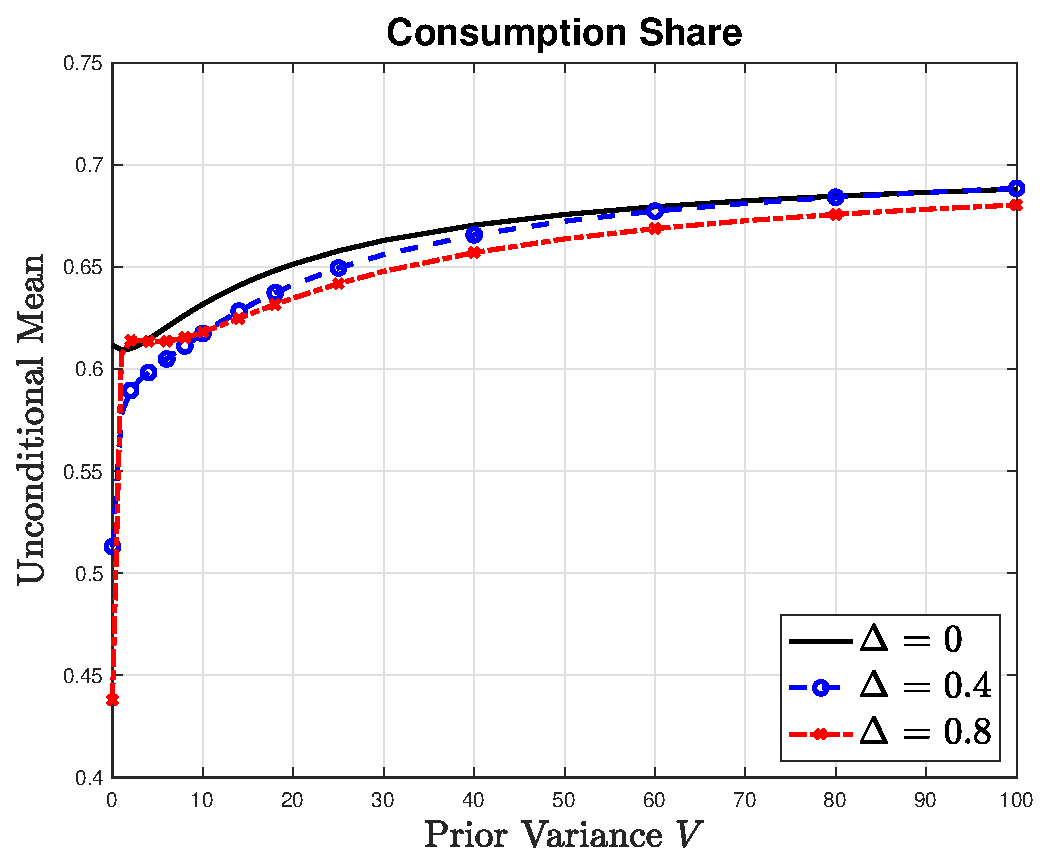
\includegraphics[width=.3\textwidth]{figures/FigLearning_f_v1.eps} &
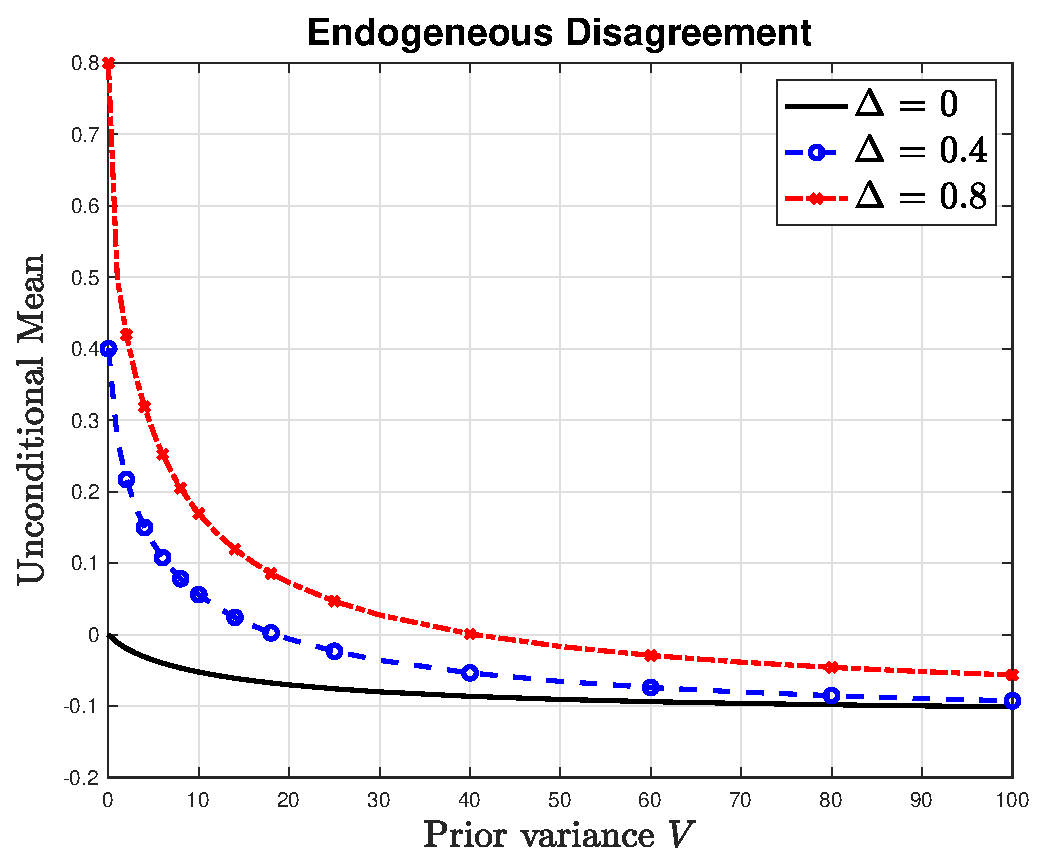
\includegraphics[width=.3\textwidth]{figures/FigLearning_DeltaM_v1.eps}
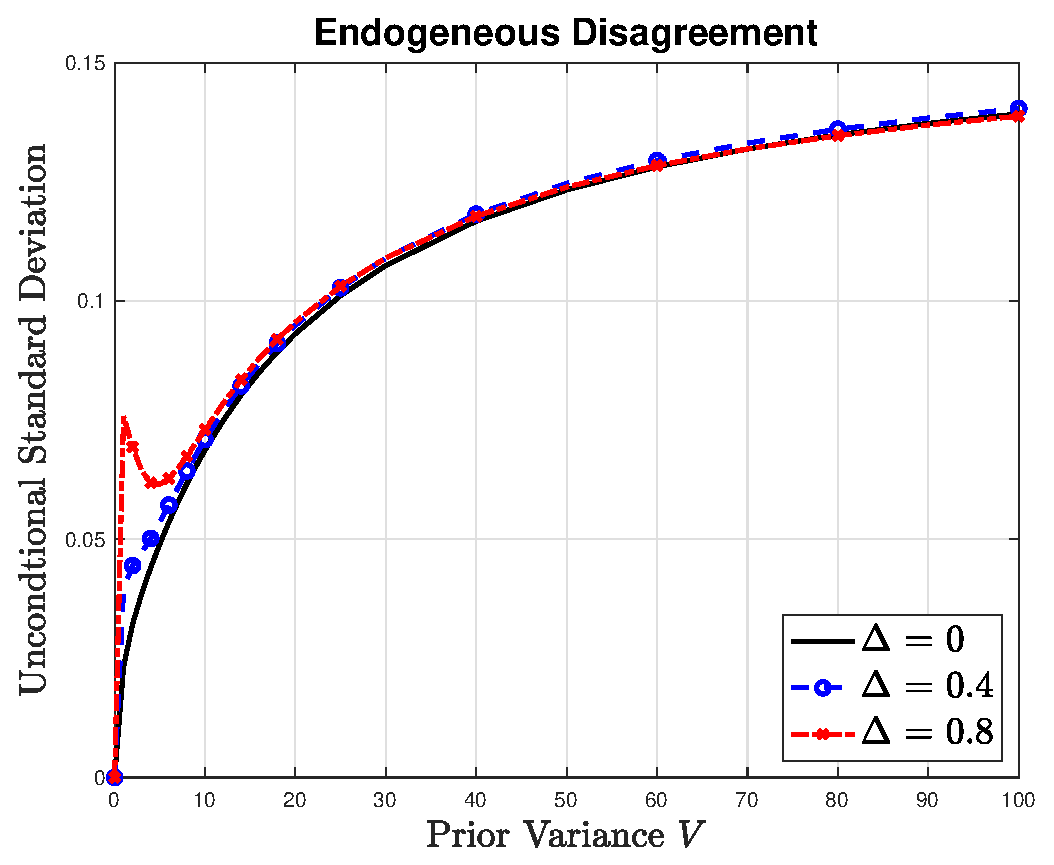
\includegraphics[width=.3\textwidth]{figures/FigLearning_DeltaSTD_v1.eps}
\end{tabular}
\caption{\emph{Unconditional moments of the consumption share and disagreement.} \footnotesize{This figure shows the unconditional mean of the consumption share (left), the unconditional mean of disagreement (middle) and the unconditional standard deviation of disagreement (right) as a function of the prior variance $V$ for different initial disagreement $\Delta$. All other parameters are as in the baseline calibration. The summary statistics are based on one million years of monthly observations for each prior variance value $V$.}} \label{CshareandDislearning} %We keep track of 12000 cohorts.}} \label{CshareandDislearning}
\end{figure}
 
The middle and right graph of Figure \ref{CshareandDislearning} show the unconditional mean and volatility of disagreement between patient and impatient investors $\Delta_t$, respectively. % given in Proposition \ref{LearningEstimationError}. 
As expected, this disagreement converges towards zero when $\Delta \neq 0$. However, this average is not zero even when all agents are born with the true prior (black solid line) because there is a correlation between the fraction of patient newborns $\alpha_t$ and disagreement $\Delta_t$. Importantly, the right plot shows that the standard deviation is increasing even for the case with no initial disagreement. This implies that ``typically'' there is more disagreement when the prior variance, $V$, is high even when the two groups start we the same beliefs. Hence, the model with learning from experience endogenously creates disagreement between the two groups of investors and as we show below implies similar asset pricing implications as the case without learning.  


Figure \ref{APlearningFIG} shows the average risk free rate (left plot), the standard deviation of the market return (middle plot) and the risk premium on the market (right plot) as we vary the prior variance $V$ for initial disagreement $\Delta=0, 0.4, 0.8$. As the prior variance increases, initial disagreement has less impact. If there is no initial disagreement ($\Delta=0$), then the standard deviation and risk premium are increasing in $V$ which implies more disagreement and so is similar to the case without learning. In contrast, the risk-free rate is decreasing with disagreement measured by V because the average consumption share of patient investors increases. 

\begin{figure}[htbp] 
\centering
\vspace{0.1in}
\begin{tabular}{ccc}
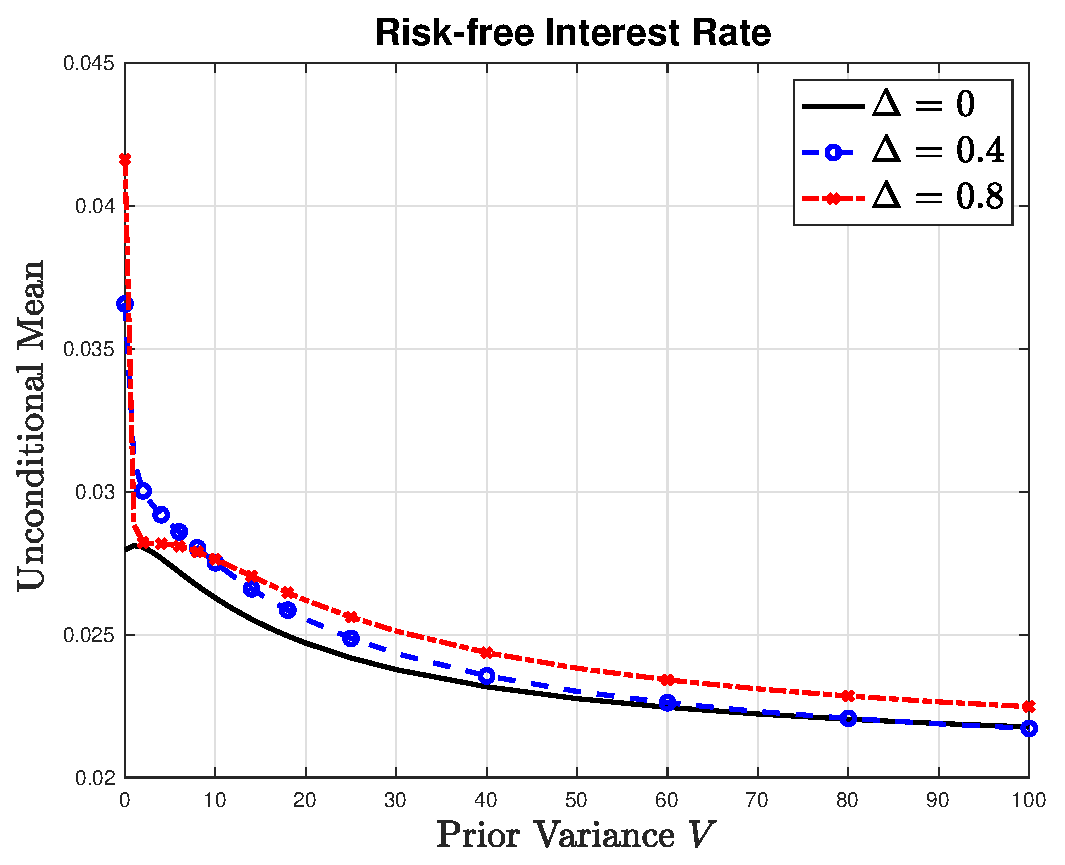
\includegraphics[width=.3\textwidth]{figures/Fig_learning_r_v1.eps} &
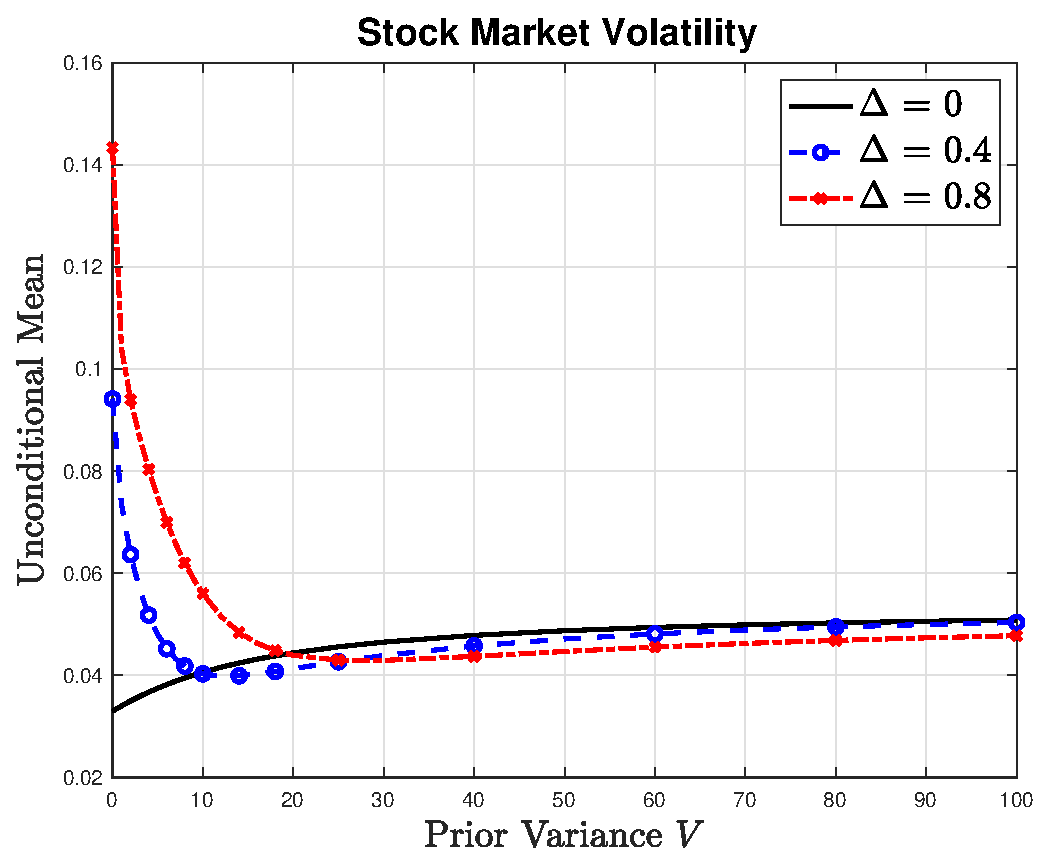
\includegraphics[width=.3\textwidth]{figures/Fig_learning_StdevRM_v1.eps}
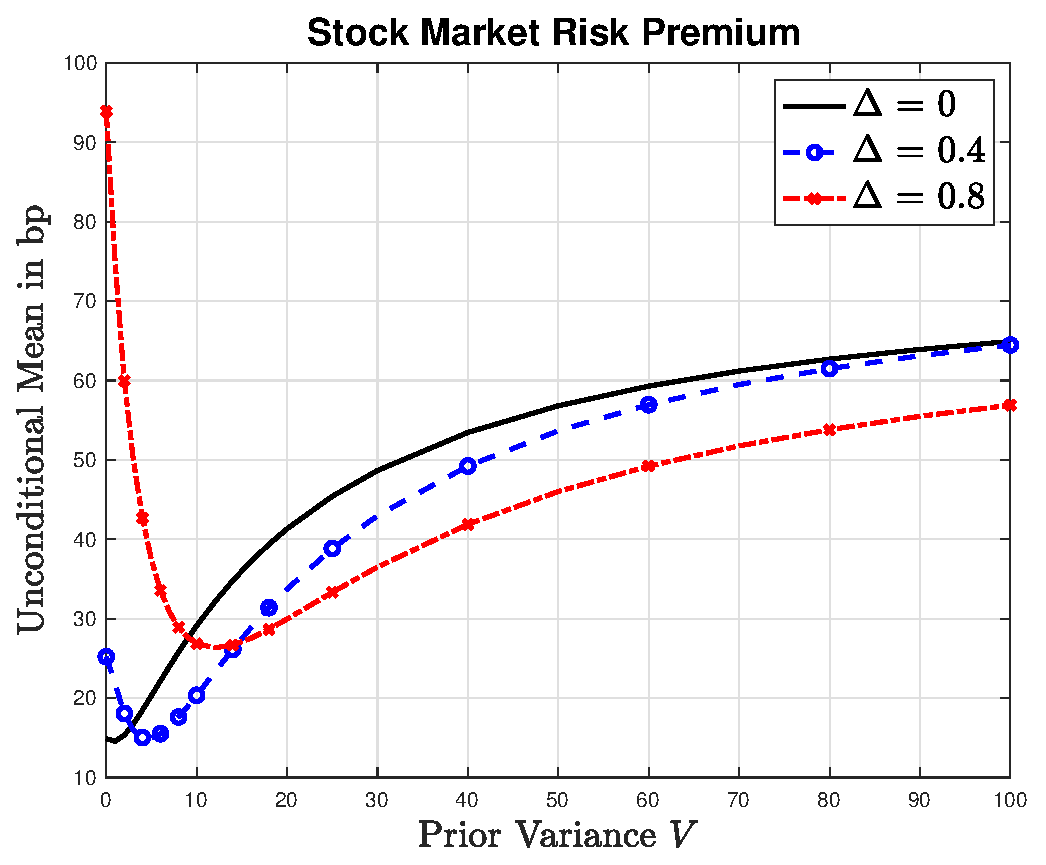
\includegraphics[width=.3\textwidth]{figures/Fig_learning_RiskP_v1.eps}
\end{tabular}
\caption{\emph{Asset pricing with learning from experience.} \footnotesize{The figure shows the unconditional mean of the risk free rate (left plot), stock market volatility (middle plot), and stock market risk premium (right plot) as a function of the prior variance (disagreement) for different initial disagreement $\Delta$ set to $0$, $0.4$ and $0.8$.  All other parameters are as in the baseline calibration. The summary statistics are based on one million years of monthly observations for each prior variance value $V$.}} \label{APlearningFIG} %We keep track of 12000 cohorts.
\end{figure}

